\section{LED et résistance (4 points)}

Lorenzo réalise le circuit suivant en utilisant une résistance de 50 $\Omega$ . \'A l'aide d'un voltmètre il mesure la tension aux bornes du générateur ($U_G$)et de la LED ($U_{DEL}$) .

\begin{center}
	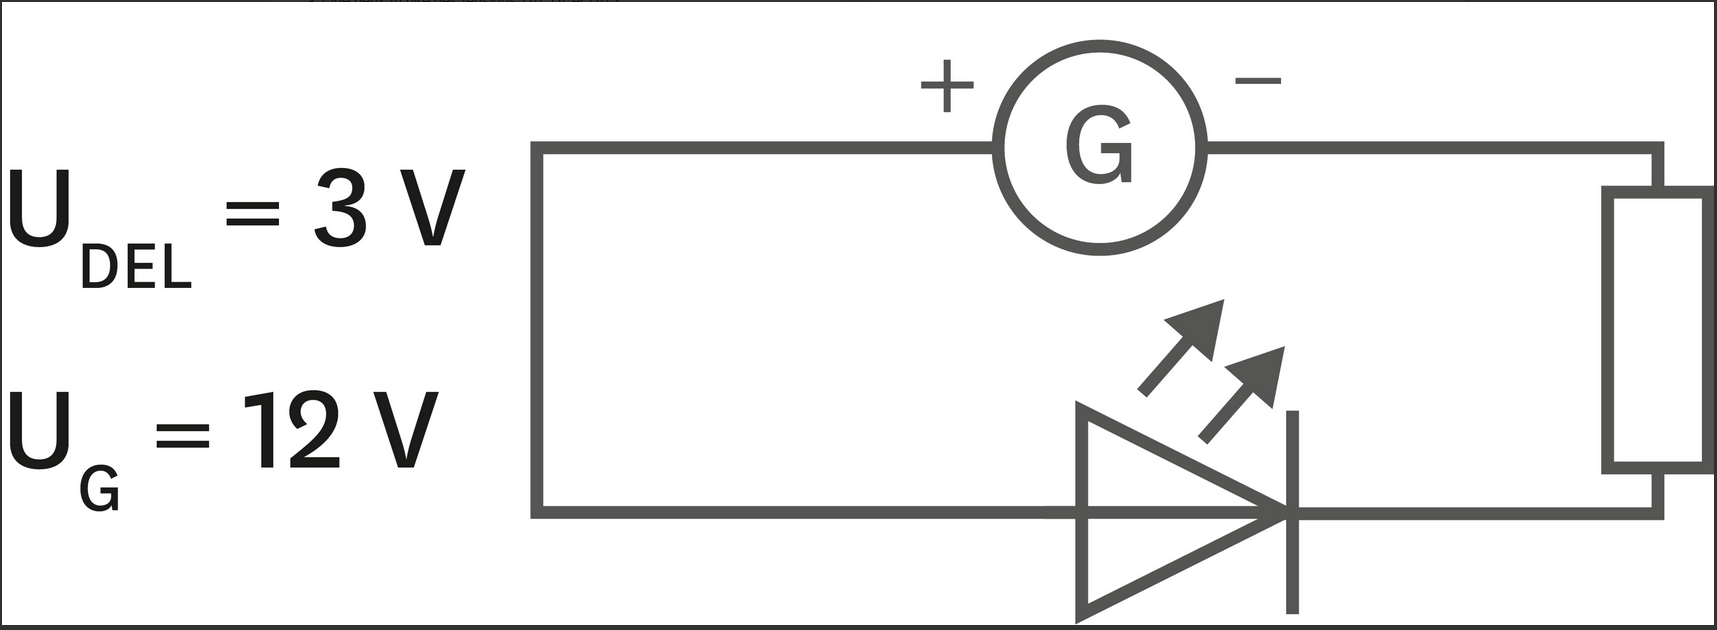
\includegraphics[scale=0.2]{img/circuit}
\end{center}

\begin{questions}
	\question[1] Comment sont branchés la LED et la résistance ?
	\begin{solution}
		La LED et la résistance sont branchées en série.
	\end{solution}
	
	\question[1] Calculer la tension aux bornes de la résistance ($U_R$) ?
	\begin{solution}
		Dans un circuit série, la tension aux bornes du générateurs est répartie entre les différents dipôles récepteurs. On a donc :
		
		\begin{eqnarray*}
			U_G &=& U_{LED} + U_R\\
			12 &=& 3 + U_R\\
			U_R &=& 12 - 3 \\
			U_R &=& 9 \\
		\end{eqnarray*}
	
	Donc la tension aux bornes de la résistance est de 9 Volts.
	\end{solution}
	
	\question[1] Calculer l'intensité du courant qui traverse la résistance ($I_R$) ?
	\begin{solution}
		D'après la loi d'Ohm, on a :
		
		\begin{eqnarray*}
			U_{R} &=& R \times I_{R}\\
			I_{R} &=& \frac{U_{R}}{R} \\
			I_{R} &=& \frac{9}{50} \\
			I_{R} &=& \num{0.18} \\
		\end{eqnarray*}
	
	Donc la résistance est traversée par un courant de 180 $mA$.
	\end{solution}
	
	\question[1] En déduire l'intensité du courant qui traverse la LED.
	\begin{solution}
		L'intensité du courant électrique est la même en tout point d'un circuit série. Donc L'intensité du courant qui traverse la LED est la même que pour la résistance, 180 $mA$.
	\end{solution}
\end{questions}